\section{Literature review}
\subsection{Introduction}
Before a computer aided detection (CAD) system for lung nodule detection can be
developed, it has to be clear what exactly has to be detected by the algorithm.
Therefore, the appearance of lung abnormalities is discussed first and a
delineation of the term 'nodule' is provided. Then an overview of commercial and
research-based CAD systems is given and a comparison of performances is
discussed. Finally, learning algorithms commonly used in CAD systems are listed
together with their merits and disadvantages.

\subsection{The biology of lung nodules}
Lung nodules are lung tissue abnormalities that are roughly spherical with a
diameter of up to 30 mm. On chest CT scans they appear as a rounded or irregular
opacity (\autoref{fig:nodules}). Many types of lung nodules can by distinguished on CT
scans. A centrilobular nodule is separated by several millimeters from the
pleural surfaces, fissures and interlobular septa. They range in size from a few
millimeters to 10 millimeters. A micronodule is less than 3 millimeters in
diameter. A ground-glass nodule -- or non-solid nodule -- appears on the CT
scans as a hazy attenuation in the lung. This type of nodule does not efface the
bronchial and vascular margins. A solid nodule shows a homogeneous soft-tissue
attenuation. Finally, a part-solid nodule exhibits both ground-glass and solid
soft-tissue attenuation characteristics \cite{nodule}.
\begin{figure}[htp]
\begin{center}
  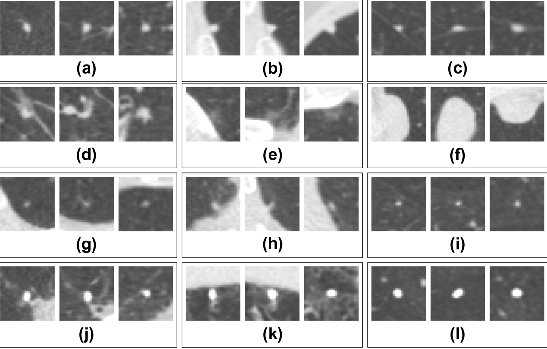
\includegraphics[width=\linewidth]{img/vanginnekennodules.png}
  \caption{In every box a nodule is shown in a sagittal, coronal and axial
  view. (a) an isolated nodule of 4.4 mm; (b) a pleural nodule of 4.2 mm; (c) a
  peri-fissural nodule of 4.8 mm; (d) a nodule of 5.9 mm with vascular attachments; (e) a ground-glass nodule of
5.4 mm; (f) a large pleural nodule (18.4 mm); (g) small nodule of 3.2 mm; (h)
small nodule of 3.5 mm; (i) small nodule of 2.3 mm; (j�l) shows three examples
of calcified nodules (indication of benign nodules) which is indicated by the
brightness of the nodules \cite{ginneken}.}
  \label{fig:nodules}
\end{center}
\end{figure}
The types of nodules stated above can be categorised. Juxta-vascular
pulmonary nodules have significant connections to their neighbouring vessels.
Pleural tail nodules have only thin connections to the neighbouring pleural
wall. Well-circumscribed nodules on the other hand do not have a connection to
the neighbouring vessels and structures. Juxta-pleural nodules show some degree
of attachment to their neighbouring pleural surface \cite{kostis}.

\begin{figure}[htp]
\begin{center}
  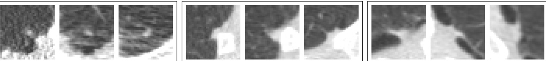
\includegraphics[width=\linewidth]{img/vanginnekenNonnodules.png}
  \caption{In the three boxes an apical scarring, a pleural thickening and a
nodular abnormality next to an emphysematous bulla are displayed in a sagittal,
coronal and axial view. These may be perceived by a nodule detection algorithm
as nodules, but in fact they are no nodules \cite{ginneken}.}
  \label{fig:Nonnodules}
\end{center}
\end{figure}

A number of nodule segmentation algorithms perform well in detecting specific
types of nodules, for example large, spherical, isolated nodules. However, these
CAD systems show large limitations in detecting e.g. non-isolated nodules that
are connected to the pulmonary wall \cite{keshani}. These algorithms can be
usefull in particular situations, but if a detection algorithms really aims at
being an asset for the radiologist, it should be able to detect all nodules
while refusing as much false positives as possible (\autoref{fig:Nonnodules}).

\subsection{Overview of existing lung nodule detection systems}
As the demand for a reliable CAD system to detect pulmonary nodules is urgent, a
lot of research has been dedicated to the matter. Several commercial systems
have already been developed and many workstations that radiologists use to
examine CT scans offer on-board nodule detection or enhancement capabilities
\cite{ginneken}. However, although a lot of efforts were made, the results shown
in the various studies are rather diverse.

\subsubsection{Commercial systems}
In 2004 iCAD, Inc., provided lung cancer detection, analysis and tracking
software for the TeraRecon's Aquarius product line. The latter licensed three
software modules from iCAD. The iCAD QuickCue\texttrademark for example
automatically detects cancerous lung nodules while the iCAD
QuickMatch\texttrademark locates, compares and tracks these nodules in previous
or subsequent patient studies \cite{tera}. However, the ImageChecker CT,
launched by R2 Technology, was the first CT Lung CAD system approved by the US
Food and Drug Administration (FDA) for the detection of lung nodules during the
examination of CT scans \cite{Mevis}. In 2005 R2 Technology, Inc., introduced
the second-generation ImageChecker CT Lung Version 2.0 CAD system which also
implemented the AutoPoint temporal comparison algorithm. This CAD system
``highlights abnormalities'' and compares new and past images to demonstrate
changes that have occured over time \cite{diag, r2}. In 2006 Vital Images, Inc.,
and R2 Technology, Inc., announced the implementation of the R2 Technology's
ImageChecker CT Lung CAD software into the Vitrea workstations \cite{vital}. In
the same year another company, Hologic, Inc., acquired R2 Technology, Inc., and
implemented their CAD technology \cite{Hologic}. Then, in 2008, MeVis Medical
Solutions AG, Inc., acquired the Pulmonary Computed Tomography Business from
Hologic R2, Inc. \cite{Mevis}.

Although the technology from R2 Technology is in high demand, some companies
have also developed their own software. In 2007 Medicsight plc announced it was
granted a medical device license from the Therapeutic Products Directorate of
Health in Canada to introduce Medicsight LungCAD API \cite{HI}.
Median Technologies offers the LMS-Lung and LMS-Lung / CAD modules which provide
quantification and detection functionalities for pulmonary (solid) nodules and
micronodules \cite{median}. And Siemens has developed the syngo.CT Lung CAD.
They claim it is ``a fully automated computer assisted second reader tool'' that
is designed to assist radiologists in the detection of solid pulmonary nodules \cite{siemens}.

\subsubsection{Publications of automated lung detection systems}
Apart from these numerous commercial systems also a lot of academic research
centra have tried to come up with a successful pulmonary nodule detection
system. \cite{review} suggest that most CAD systems for the automated detection
of lung nodules proceed according to a number of steps of which the first one is
the acquisition of data. The detection of lung nodules is preferably performed
on CT scans as they enable the visualisation of small volume and low-contrast
nodules because of the limited slice thichness. A large number of chest CT scans
are available in public databases such as the LIDC database. During the next
step, the data are pre-processed to remove noise and artefacts. This might
improve the quality of the images, but it is not necessary to do so. In the
third step a segmentation of the lungs is performed. The lung lobe region is
identified and the rest of the image is removed. This reduces the computational
cost compared to the case where the whole image is processed and it increases
the reliability, the accuracy and the precision of the algorithm. This
increases the performance of the next step: the nodule detection. ``Lung nodule
detection refers to the process of determining whether nodule patterns are
present in the image and identifying the location of the nodules''
\cite[p.~154]{review}. Nodule detection methods can be categorized according to
the detection method that is applied. The first group of publications uses a
classification technique to classify voxels or regions of interest (ROI). In
addition, a clustering method may be implemented to improve the performance of
the automated nodule detection method. The second group uses template matching
to detect specific geometries. The third group relies entirely on the output of
a lung nodule segmentation method. The systems that include a classification
component in their nodule detection algorithm have demonstrated better
performances \cite{review}. In the final step, the amount of false positives is
reduced to achieve a maximum sensitivity. In the following paragraphs a summary
of relevant literature is given.

The first problem that arises when laymen start processing CT scan in search
for nodules is that they have to rely on the annotations made by expert
radiologists. Accurate delineation of these lung abnormalities is crucial for
optimal image analysis. The current approach to delineate lung nodules in CT
scans involves one or more radiologists manually drawing the boundaries of the
nodules. Often this manual segmentation overestimates the nodule volume to
ensure the entire lesion is enclosed \cite{rex}. Furthermore, this process is
highly variable \cite{cooper}. But the success of the extraction of image
features depends on the accurate delineation of the nodules. Therefore, if one
wants to develop a nodule segmentation method -- or any other nodule detection
method -- it is of utmost importance this delineation is done in an accurate and
reproducible way. \cite{gu} have improved the ``Click and Grow'' algorithm that
has been developed by Definiens AG and Merck and Co., Inc., which
semi-automatically isolates tumors in CT images. The idea is that a radiologist
detects the nodule and clicks on the region of interest in a 2D slice. This
click initiates multiple seed points in a certain area. Then the application
builds out the object three-dimensionally by region growing. An ensemble
segmentation is obtained from the multiple regions that were grown. An
evaluation on a set of 129 CT scans using a similarity index (SI) was performed.
The average SI was above 93\% which shows stability of the algorithm. The
average SI for two different readers was 79,5\%.

Apart from improving the manual nodule delineation of the radiologists, an image
processing algorithm may also increase their detection rate by assisting as a
``second reader''. \cite{roos} assessed the diagnostic performance of
radiologists -- with their years of experience ranging between 9 and 24
years -- using incremental CAD assistance and their temporal variation.
20 scans containing 190 non-calcified nodules with a magnitude of 3 mm and above
were examined by three radiologists. After a free search the radiologists
independently evaluated a number of CAD detections per scan. The
average sensitivity of their free search was about 53\% (range, 44\% - 59\%) at
1,15 false positives (FPs) per scan. This increased up to 69\% (range, 59\% -
82\%) and a FP rate of 1,45 per scan when using the CAD assistance. The
increase in sensitivity, with only a minimal increase in FPs, was
significant during a time period of 100 seconds. Then the increase in
sensitivity flattened from 14\% to only 2\%. This evolution was due to the fact
that the CAD nodules were presented to the radiologists in order of CAD score
and was not due to a temporal change in the readers' performance. However, it
was also noticed in this study that different readers may experience a variable
benefit from the use of CAD as some readers tend to often reject true positive
CAD candidates. This reduces the potential benefit of CAD assistance.
Nevertheless, \cite{roos} states that CAD has the potential to equalise
performance among readers by reducing individual detection errors.

\cite{elbaz} proposed a three step algorithm to isolate lung nodules from
spiral chest low-dose CT (LDCT) scans. In the first step the lung tissues were
isolated by applying an iterative Markov-Gibbs random field (MGRF) based
segmentation framework. To retain the nodules attached to the pulmonary walls, the
segmentation was refined by the iterative conditional mode relaxation that
maximizes a MGRF energy. Then the lung nodules, arteries, veins, bronchi and
bronchioles were separated from the rest of the tissues in the slice. In the
second step the lung nodules (2-12 mm) were detected by applying 3D and 2D
templates which describe typical geometry and greylevel distributions within
nodules of the same type. Four template shapes were used: solid sphere, hollow
sphere, solid circle and solid semicircle. The radius and the greyscale
intensity of the templates was made adaptable. The detection combined the
normalized cross-correlation template matching and a genetic optimization
algorithm. The third step eliminated the false positive nodules using three
textural and geometric features that were calculated for each detected nodule.
To distuingish between FPs and true positives (TPs) Bayesian supervised
classifier learning statistical characteristics from a training set (20 FP, 20
lung TP, 20 lung wall TP nodules) of nodules selected from 50 separate subjects.
CT scans from 200 subjects were used in this study. The sensitivity was 82,3\%
and a FPs rate of 9,2\% (i.e. the number of FPs (12) with respect to the
total number of true nodules (130)). The algorithm, that was implemented
in C++ on an Intel dual processor with 16 GB memory and 2 TB hard drive, took about
5 minutes to process 182 CT slices of size 512 x 512.

Other studies rely on a nodule segmentation method to detect lung abnormalities.
\cite{kuh} applies morphological opening, erosion, thresholding, seed
optimisation and boundary refinement operations to extract large nodules.
\cite{itai} proposes a segmentation of the lung areas using SNAKES method which
is an active contour model. Abnormal shadow areas including ground-glass opacity
or lung cancer over the size of 5 mm are classified by using voxel densities.
The algorithm was applied on 9 CT scans and a TP fraction of 0,81 and
a false negative (FN) fraction of 0,2 were obtained.

A third category of nodule detection methods are the classification based
methods. The main difference in output between a classification
based detection method and a segmentation method is that the latter will provide
the user with a delineation of the entire nodule, while the former will give a
nodule-probability per voxel. \cite{ozekes} tested four different learning based classification
methods: a Neural Network (NN) classifier, a Support Vector Machine (SVM)
classifier, a Naive Bayes classifier and a logistic regression classifier. First
ROIs were extracted by applying thresholding and an 8-directional search in which
candidate lung nodule voxels have to have neighbour voxels with densities
between a minimum and maximum density threshold. From these ROIs a number of
features were extracted: straightness, thickness, vertical and horizontal
widths, regularity and vertical and horizontal black pixel ratios. These
features were then fed to the four classifiers. The NN classifier
showed the best results, followed by the SVM classifier. \cite{keshani} also
applies an SVM classifier and active contour modelling to detect lung nodules.
The lung area was first segmented by active contour modelling which was followed
by a set of masking techniques to transfer nodules from non-isolated into
isolated ones. Based on a set of 2D and 3D features the SVM classifier detected
the lung nodules. Then the contours of these nodules were extracted
by active contour modelling. In a last step the lung tissues in the original
image were classified into four classes: lung wall, parenchyma, bronchioles and
nodules. The results from this classification were used to distuingish solitary
nodules from attached ones. When this algorithm was used to detect nodules in
the ANODE09 dataset an average detection rate of 37,8\% was obtained while the
best performing method yielded a detection rate of 63,2\%. The latter algorithm,
ISI-CAD, was developed by \cite{mur} and uses the local image features -- shape
index and curvedness -- to detect candidate nodules. Two successive k-nearest-neighbour
(K-NN) classifiers are applied to reduce the number of FPs. This
yielded a sensitivity of 80\% with an average of 4,2 FPs per scan.
\cite{sluimer2003} also used k-NN for developing an algorithm which
automatically distuinguishes between normal and abnormal lung tissue.
Before k-NN was applied, a principal texture analysis was performed in this
study to determine local features.


In addition to applying a classification based detection method, a clustering
method can be implemented as well to improve the performance of the classifier.
\cite{kawata} developed a linear discriminant classification boosted by k-means
clustering method to distuingish between malignant and benign nodules based on
topological histogram features. The k-means clustering divided the datasets of
nodules in homogeneous classes to improve the performances of the  linear
discriminant classifier. \cite{lee2010} also applied an ensemble classification
aided by clustering (CAC) method. First, nodule and non-nodule parts of a
training set were merged and then clustered into M clusters to take advantage fo the
similarity among features of nodule and non-nodule instances. Then each cluster
is divided into two groups, namely nodules and non-nodules. Then a multi-class
classifier was trained consisting of 2xM classes. The classifiers used were a
Random Forest (RF) classifier, a SVM classifier and a
Decision Tree (DT) classifier. There were two different clustering methods
applied: k-means and expectation maximisation (EM). The best results were
obtained by the RF CAC EM algorithm. It yielded a classification accuray of 97,72\% while
SVM and DT CAC EMs recorded 96,46\% and 93,98\% respectively on the same
dataset. However, the execution time of the SVM CAC EM algorithm was the lowest
(182 seconds). These results were compared to non-CAC methods.
The highest classification accuracy of 95,64\%, a sensitivity of 95\%, a
specificity of 96,28\% and a FP rate of 3,72\% were obtained by
non-CAC RF. This method also recorded the lowest execution time (10 seconds).


\subsubsection{Performance of existing systems}
 The algorithms presented in a wide range of papers report varying
 successes in the automated detection of nodules. However, it is very difficult
 to compare studies against one another in a meaningful way due to differences
 in the size of the datasets, the evaluation methods, the data selection
 criteria and the characteristics of the nodules \cite{lee2010}. Especially
 comparing older and contemporary studies is difficult as older ones may have
 used scans with thicker sections (range 2.5 - 10 mm), on which small nodules
 are rather difficult to detect, than the scans nowadays (2,5 mm) \cite{lee2010,
 ginneken, mur}. Some studies focus on nodules below or above a certain
 size or on special types of nodules (e.g. solid nodules). \cite{mur} performed an extended
 literature review and found that the number of scans used for testing varied between 5 and 500 with a
 median number of 29,5. Many of the studies included multiple scans from
 individual patients, which means that the diversity of the available nodules
 was reduced. Furthermore, the results of publications are often presented in
 diverse ways. \cite{results} suggests the performance of CAD systems should be
 presented a the sensitivity of the system, the specificity, the accuracy, the
 error rate, the TP rate and the FP rate. %TODO fix
 
%TABEL X GEEFT OVERZICHT WEER VAN BEST AND SLECHTS PRESTERENDE ALGORITHMS BASED
% ON EXHAUSTIVE LITERATURE REVIEW ??
 
 In order to improve the access to data, and thereby the comparability between
 studies, the Lung Image Data Consortium (LIDC) created a publically available
 database which provides researchers with a vast amount of test- and
 trainingsdata. Nevertheless, as one can take different subdatasets from this
 large database for the training and the testing of algorithms, it is still not
 possible to compare results in an objective and meaningful way. Therefore,
 \cite{ginneken} created ANODE09, a database of 55 scans and a web-based
 framework which allows researchers to test their algorithms and to
 compare results against one another.
 




